\section{Introduction to Computer Vision}
\subsection{What is Computer Vision?}
\begin{flushleft}
    \large \textbf{Computer vision} is a field of machine learning that focuses on enabling computers and programs to \lq see' images. \lq Seeing', in this case, defines a computer's ability to recognize and understand objects in images, such as a program \lq seeing' a dog and labeling it as such. Computer vision is used in many ways, most commonly utilized for \textbf{object detection, image classification, and segmentation} (a process of breaking an image down to identify boundaries of objects and objects themselves).  We will primarily be covering where computer vision instersects with deep learning, but do note that computer vision as a field has existed well before deep learning and there are many aspects of the field that are more algorithm based than AI based.
\end{flushleft}

\section{Convolutional Neural Networks}
\begin{flushleft}
    \large Now what machine learning algorithm is used for computer vision? That would be \textbf{Convolutional Neural Networks} or \textbf{CNNs}. CNNs are designed to process images and can either be found as independent models or as parts of other neural networks. They can work as image pre-processors for other models, like multimodal language models. Similar to how neural networks were designed to mimic brain functionality, CNNs are designed to \textit{mimic a human's visual processing system} and the brain's visual cortex. 

    \subsection{Convolutional Layer}
        Convolutional neural networks are structured as a series of layers, similar to neural networks. The first layers are called the \textbf{convolutional layers}. Convolutional layers apply a mathematical calculation to a section of an image to extract information about the features in that image. Recall that a feature is an attribute of interest, such as an ear, number of legs, presence of color, etc. It does this using an object called a \textbf{kernel}. A kernel works like a sort of filter, amplifying the effect of some pixels and minimizing the effect of others to try and draw out a feature. For example, the kernel in the image below is attempting to extract an ``ear'' feature from a section of the input image. 
        \begin{figure}[H]
            \centering
            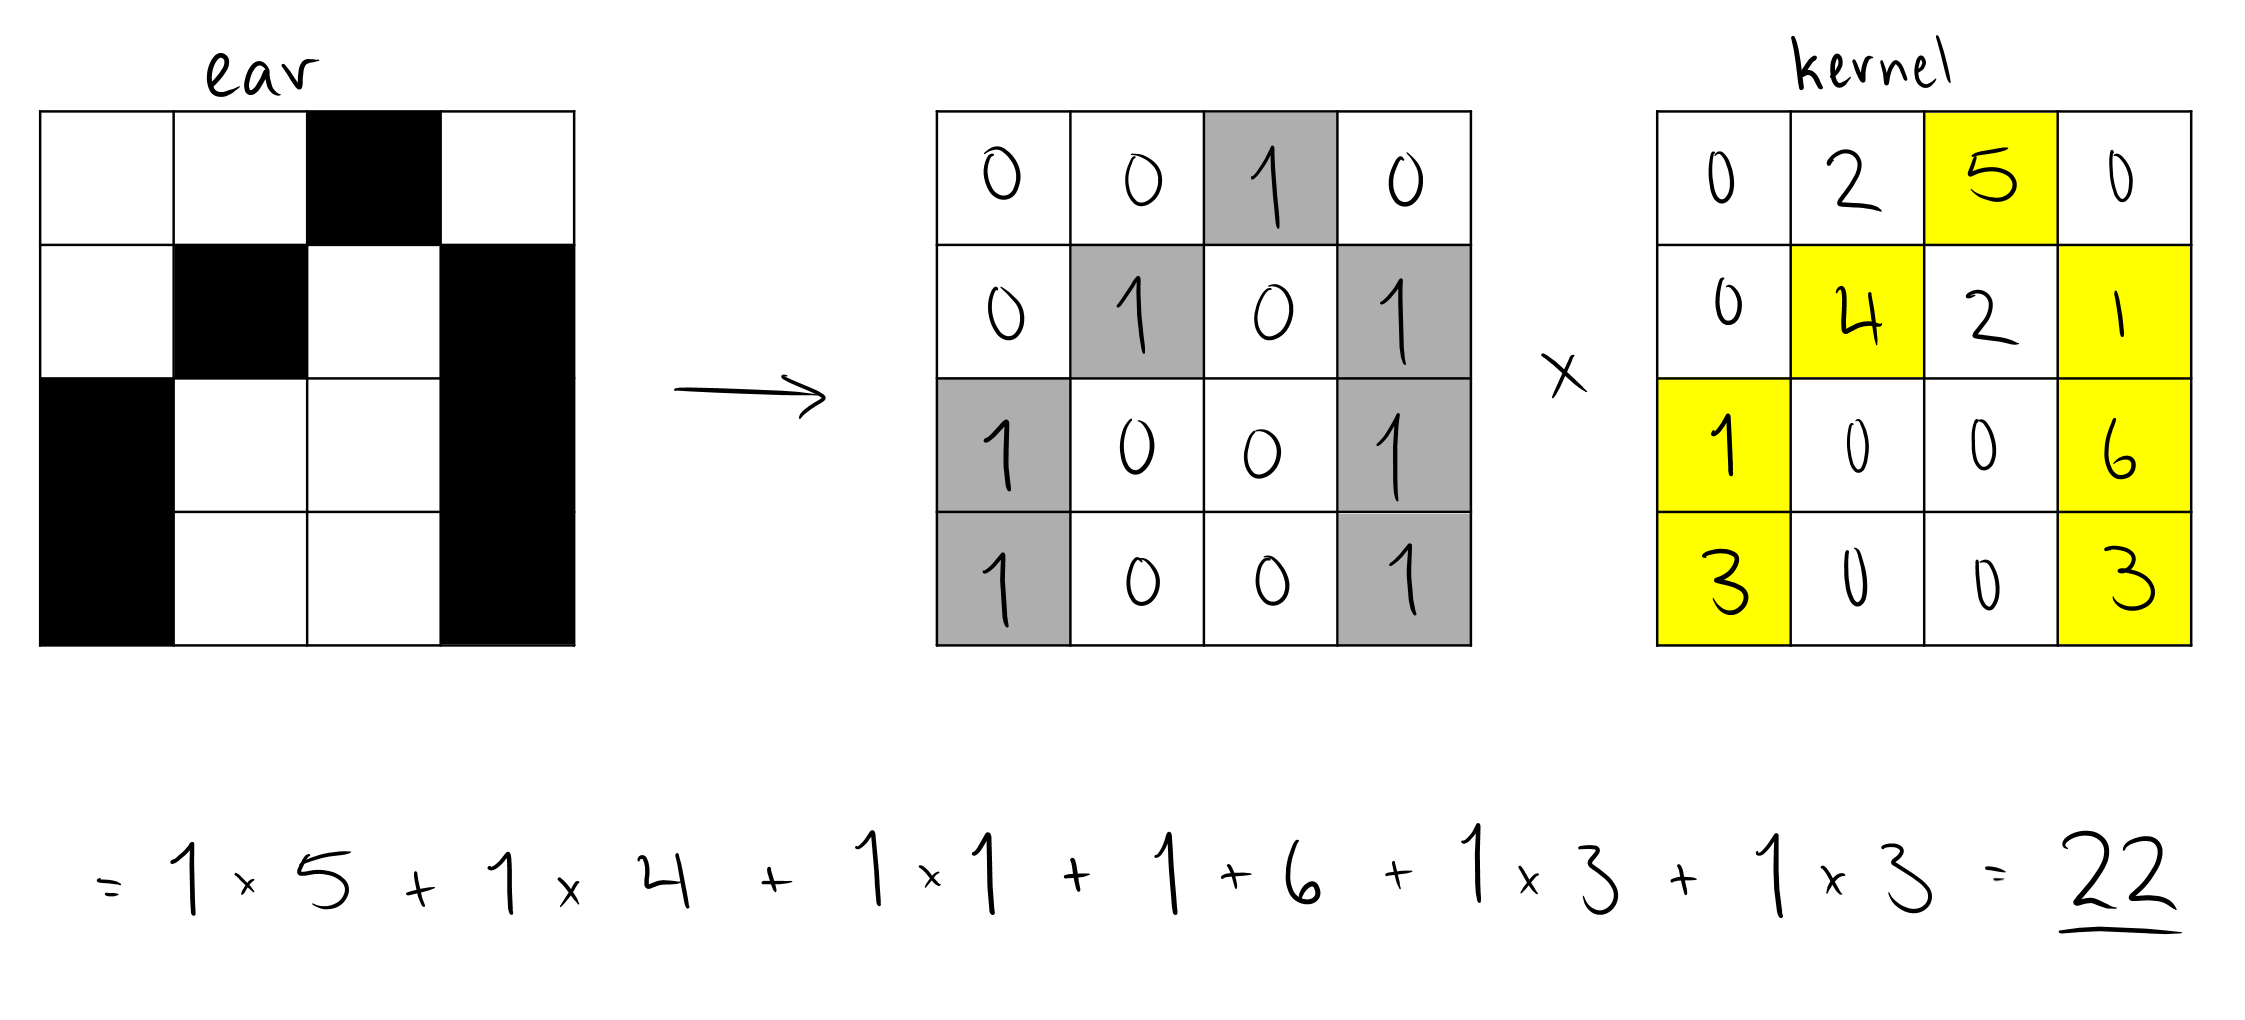
\includegraphics[width=1\linewidth]{cv/kernelextraction.png}
            \caption{Illustration of feature extraction using kernel}
            \label{fig:kernelextraction}
        \end{figure}

        The solution to the calculation is then placed back into a new, usually smaller, matrix that will ultimately become a representation of where the features we are searching for within the image exist. We call this a \textbf{feature map}. For example, if there is an ear in the top left of an image, then an ``ear'' kernel applied to that image will result in a feature map that has high values in the top left where the ear was. 

        \begin{figure}[H]
            \centering
            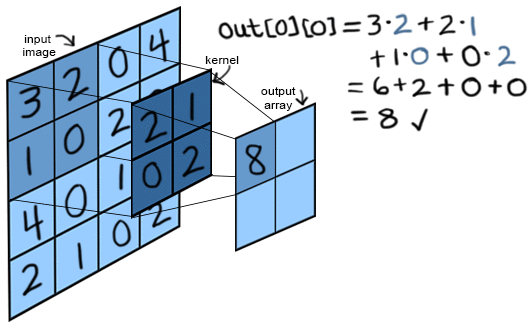
\includegraphics[width=0.75\linewidth]{cv/imagetokerneltosmallmatrix.png}
            \caption{Illustration of the work done in a convolutional layer}
            \label{fig:imagetokerneltosmallmatrix}
        \end{figure}

        The formula for the convolutional layer's calculation is a dot product calculation, where a filter (a.k.a kernel) $F$ is applied to an image in sections (the number of sections depends on the size of the image and the size of the filter) as seen below. We will use the image above for examples as we break down the equation.
        
        $$Z(i, j) = \sum^{k-1}_{m=0} \sum^{k-1}_{n=0} \sum^{C}_{c=1}  I(i+m, j+n, c) \cdot F(m, n, c) $$
        
        The variables $i$ and $j$ denote where in the image we are looking at the moment. If we input $(0,0)$, the top left of the filter would be placed at $(0,0)$. This is what is happening in the above figure. \break
        
        The size of the filter is an $k \times k$ matrix (a $2 
        \times 2$ matrix in the above figure). So when we place it on the image, we get an $k \times k$ ``focus zone'' where we are looking for a feature. \break
        
        $m$ and $n$ within the summations denote the coordinates of pixels in both the image $I$ and the filter. We iterate through them, multiplying the pixel value of a coordinate within the image by the value within the filter that ``overlaps'' it. You can see this being done in the above image, as we multiply the pair $3 \times 2$. The 3 comes from the image and the 2 comes from the overlapping spot in the filter. We repeat this for all pixels in the ``focus zone'', summing them all up.\break
        
        The coordinate $c$ designates the \textbf{channel} of the image and filter the calculation is currently focusing on. Colored images have 3 channels, one that stores the R (red) pixel value, one that stores the G (green) pixel value, and one that stores the B (blue) pixel value. We would apply a filter to each of these channels separately. This allows us to detect features through the dimension of color as well (e.g. ``red ear''). The filters applied to each channel can be the same, or different, depending on the architecture of the CNN. There are also other encodings for colored images, such as HSV or CMYK. Black and white images can be encoded in just one channel.\break
        
        Finally, $Z(i,j)$ returns the value  that we will store in the feature map described previously. \break

        Along with kernels, two other factors affect how the feature map $Z$ is created, \textbf{stride} and \textbf{padding}. Stride denotes how many pixels the filter is shifted by during the calculation. The kernel can be shifted by only 1 pixel meaning there will be overlap in the sections of the image the kernel is placed on. Or, with a stride that equals the width of the kernel, the sections that the kernel is applied to do not overlap. In the above image, the stride is 2. Observe more examples of strides that are depicted in Figures 3 and 4 below. 

        \begin{figure}[H]
            \centering
            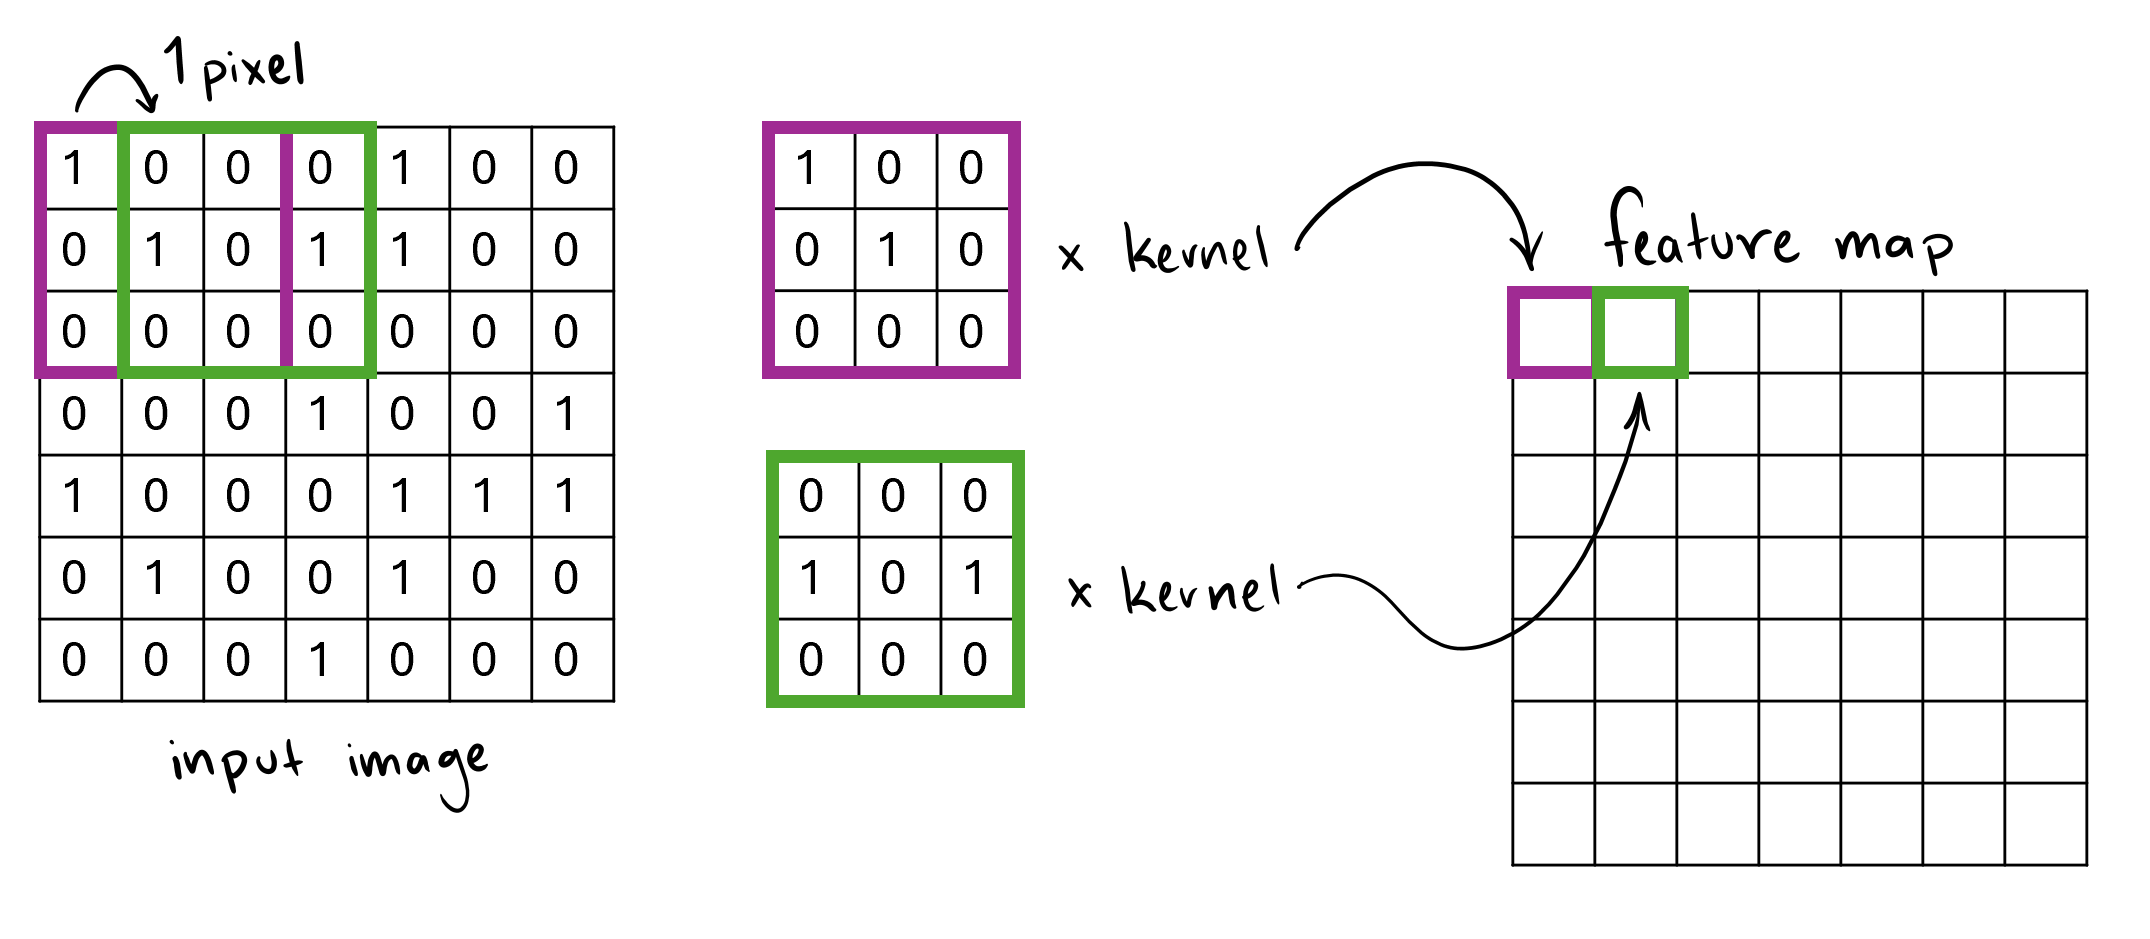
\includegraphics[width=1\linewidth]{cv/stridedepict.png}
            \caption{Illustration depicting a stride of 1 pixel}
            \label{fig:stridedepict}
        \end{figure}

        \begin{figure}[H]
            \centering
            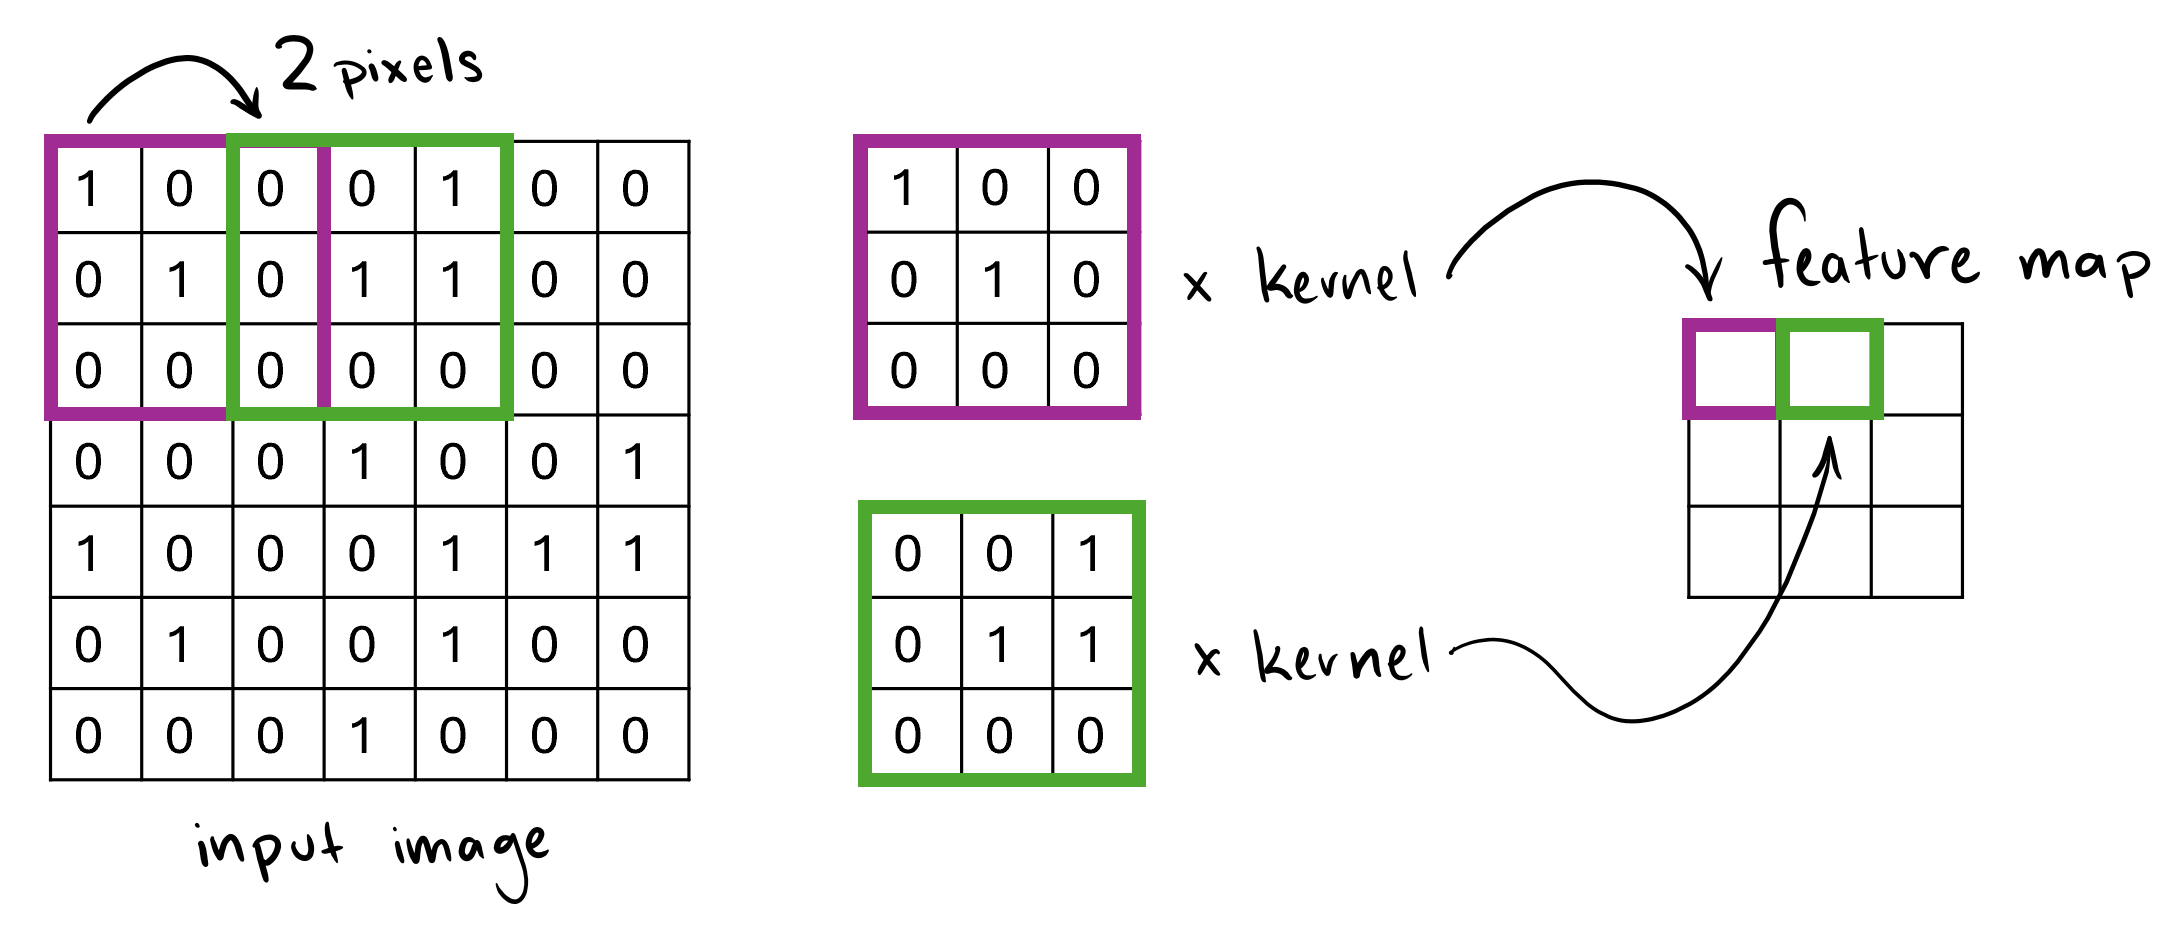
\includegraphics[width=1\linewidth]{cv/stride2eg.png}
            \caption{Illustration depicting a stride of 2 pixels}
            \label{fig:stride2eg}
        \end{figure}

        Padding, on the other hand, refers to extra pixels around the edges of a kernel. These extra pixels, usually having a value of 0, control the size of the outputted feature map. With padding, we can manipulate the size of the feature map in multiple ways, including leaving the feature map with the same dimensions as the input matrix, while still applying the kernel as a filter.

    \subsection{Nonlinearity in CNNs}
        CNNs, like all neural networks, employ \textbf{nonlinearity} to model the complex patterns in their data that cannot be captured by linear transformations alone. Nonlinearity is vital for neural networks - without it, all their calculations would be the equivalent of a single linear operation. Using non-linear functions break this linearity, enabling the model to approximate complex, non-linear decision boundaries, which is essential for tasks like image recognition, object detection, and natural language processing. In CNNs, this nonlinearity is employed after the application of the kernel and with \textbf{activation functions}. Using non-linearity after convolutional layers aids the network in learning hierarchical features of increasing complexity. Early layers learn simple features like edges and textures, while deeper layers combine these to detect more abstract features such as objects or shapes. \break

        CNNs commonly use the \textbf{Rectified Linear Unit or ReLU} activation function. ReLU, as seen in the formula below, is quick, efficient, and requires little computation power. 
        
        $$ReLU(x) = \mathrm{MAX}(0,x)$$
        
        ReLU leaves all positive values unchanged and changes all negative values to 0. This method prevents certain neurons from activating, making the model more efficient and less prone to overfitting. However, stopping neurons from activating also has disadvantages, such as certain features or neural connections `dying out'. This means some neurons will never learn and advance, since their gradients are reset to 0 using this activation function. \break

        In order to address these disadvantages, models sometimes use \textbf{LeakyReLU}. LeakyReLU uses the formula:

        \[f(x)= 
        \begin{cases}
            x,& \text{if } x > 0\\
            \alpha x, & \text{if } x \leq 0
        \end{cases}
        \]

        where $\alpha$ denotes a small positive constant, usually 0.01. In this activation function, negative values are suppressed instead of reset. So neurons will be able to activate, but their activation will be quieter and negative values will continue to have less effect on the final conclusion.

    \subsection{Pooling Layer}
        \large Now, after the convolutional layer, the features in the image are amplified and complex calculations have been used to manipulate the image to extract details from it. Once those calculations are complete, another layer manipulates the image further, summarizing all these little details brought out by the convolutional layer. This is called the \textbf{pooling layer}. The pooling layer simplifies the feature map outputted by the convolutional layer, while retaining the significant features. This reduces the amount of parameters that move on to the next layer and the amount of computation necessary, making the model more efficient. Any further operations done by the model will be done on the `pooled' matrix, with features summarized and simplified through the use of a 2-dimensional filter. For a feature map having dimensions $h \times w \times c$, the dimensions of the map after pooling would be 
        $$\biggl( \frac{h - f + 1}{s} \times \frac{w - f + 1}{s} \times c \biggr)$$
        Note that $f$ is the size of the filter used and $s$ denotes the length of the stride used. \newline

        A common technique used for the pooling layer is \textbf{max pooling}. This operation takes the maximum value in a given section of the feature map and selects that number to represent the section in the summarized map, as seen in the figure below. 

        \begin{figure}[H]
            \centering
            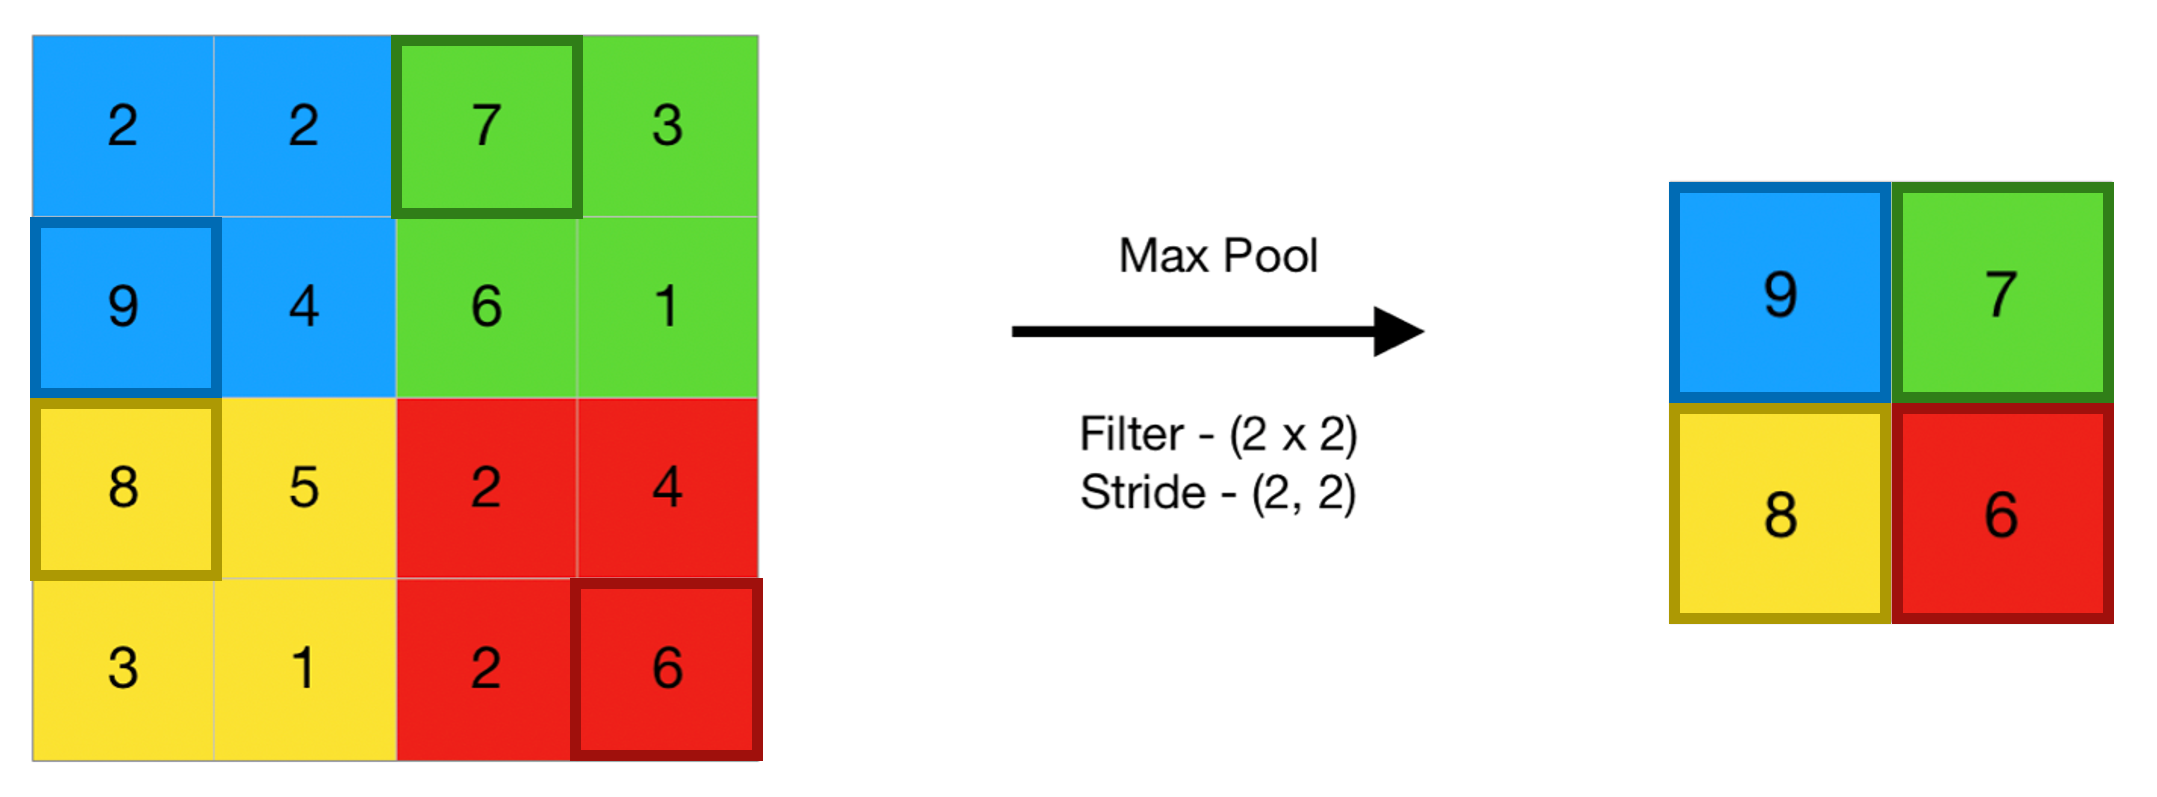
\includegraphics[width=0.75\linewidth]{cv/maxpooling.png}
            \caption{Illustration of the max pooling operation}
            \label{fig:maxpooling}
        \end{figure}

        If we take the section of the map that the max pooling operation is being done on as $Z(i, j)$, we get the following formula for the calculation on $Z(i, j)$. This calculation is done assuming a section size of $2 \times 2$.
        $$Z_{pool}(i, j) = \max \{Z(2i,2j), Z(2i+1,2j), Z(2i,2j+1), Z(2i+1,2j+1)\}$$ 

        \textbf{Average pooling}, another pooling operation, uses a similar methodology. Rather than taking the maximum value however, average pooling chooses the average value of the section rather than the maximum as representation in the pooling matrix. It's $Z_{pool}$ formula for a $2 \times 2$ section is as follows
        $$Z_{pool}(i, j) = \frac{1}{4} (Z(2i,2j) + Z(2i+1,2j) + Z(2i,2j+1) + Z(2i+1,2j+1))$$

        While pooling layers are extremely beneficial in making models more efficient, they have a few disadvantages. As you can see in both the max and average pooling operations, pooling causes significant information loss. Pooling layers minimize the data, meaning we lose information in the process. This loss can cause excess `smoothing' of the image, where finer details are lost.

        \subsection{Fully Connected Layer}
        The \textbf{dense} or \textbf{fully connected layer} is the last layer of a Convolutional Neural Network. Typically, CNNs employ several convolutional and pooling layers before the dense layer, to extract and identify all the necessary features before making a conclusion. Before the input from the last convolutional or pooling layer can be passed to the dense layer, it is flattened into a one-dimensional vector. These dense layers are just neural networks, and, in the cases where the CNN is integrated into another network, they are the neural network processing the features extracted by the CNN. The fully connected layers, or the model in the other case, perform regression or classification operations on the given input to draw a conclusion based on the data. For a single-dimensional input vector $\textbf{x}$, a weight matrix $\textbf{W}$, and a vector of bias terms of each neuron $\textbf{b}$, the formula for the vector of outputs $\textbf{z}$ would be
        $$\textbf{z} = \textbf{W} \cdot \textbf{x} + \textbf{b}$$

        The dense layer also typically uses an activation function when doing a multi-level classification operation. This activation function takes the logits from the previous layer and converts them into probabilities between 0 and 1. The \textbf{softmax activation function}, as seen below, is typically used for this specific operation. 
        
        $$\mathrm{Softmax}(z_i) = \frac{e^{z_i}}{\sum^{n}_{j=1} e^{z_j}}$$
        
        In the formula, $z_i$ denotes the raw logits calculated by the dense layers for class $i$. After applying the softmax operation to raw logits (can hold any numerical value), we get a ``probability distribution'' over all classes. We then select the one with the highest probability, and say that the image given to the CNN belongs to class $i$.

        \subsection{Loss Functions, Optimizers, and Regularization}
        Similarly to neural networks, CNNs also use loss functions, optimizers, and regularization to improve their accuracy. They use many of the same functions that we've covered already, such as \textbf{Cross-Entropy Loss} and \textbf{Mean Squared Error} for loss functions, \textbf{gradient descent} for optimization, and \textbf{dropout} for regularization. \break

        See the figure below for an overview of the entire architecture of a Convolutional Neural Network.  \break
        
        \begin{figure}[H]
            \centering
            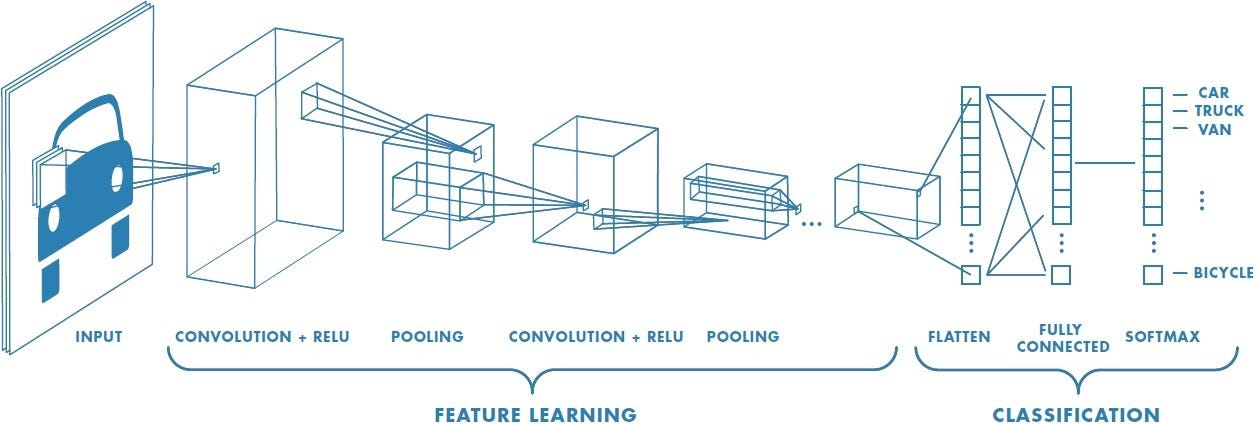
\includegraphics[width=1\linewidth]{cv/full_cnn.png}
            \caption{Illustration of complete architecture of CNN}
            \label{fig:full_cnn}
        \end{figure}
\end{flushleft}

\vspace{10px}
\begin{questionbox}
    \textbf{Synthesis Questions:}
    \begin{enumerate}    
        \item What region of the brain are CNNs (loosely) based off?
        \item Describe, in your own words, what is the purpose of a convolutional layer?
        \item What changes the size of the output feature map, padding or the values populating a kernel?
        \item What changes the values in the output feature map, padding or the values population a kernel?
        \item Why are there usually multiple convolutional and pooling layers in CNNs?
    \end{enumerate}
    \vspace{1px}
\end{questionbox}

\section{Self-Supervised Learning}
\begin{flushleft}
    \large \textbf{Self-supervised learning} or SSL, is a paradigm of machine learning that allows models to learn from useful representations of data. This means that models using SSL don't need large, extensively labeled datasets (datasets that are usually labeled manually), saving time and resources. By employing self-supervised learning, models are able to use unlabeled data to learn. The fundamental idea of self-supervised learning is for the model, when given unlabeled data, to generate labels for said data. These labels will be used as ground truths (like true labels) in further operations. In the first step, the model attempts to identify patterns in the data and then, based on these patterns. assigns labels to the data it feels confident about. Then the model continues its training, using its labels and continuing to learn with backpropagation as normal. The only difference in the training process is that every time the model makes a forward pass, it reassigns the labels to whatever data is it confident about. there are several methods SSL models employ to efficiently and reliably conduct this process.
\end{flushleft}
\subsection{Methods of SSL}
\begin{flushleft}
    \large The first method we will discuss is \textbf{Contrastive Learning}. This is one of the core techniques of self-supervised learning. Contrastive learning works to train the model to distinguish between similar and dissimilar points. Using this training, the model can determine which points should have the same label and which should have different labels. \newline  
    
    To implement contrastive learning, the model typically uses pairs or groups of data points. For example, in image data, the model might be given two views of the same image with slight transformations—like rotations, cropping, or color adjustments—as "positive" pairs. It then receives unrelated images as "negative" pairs. The model is trained to bring the positive pairs closer together in its internal representation space while pushing the negative pairs further apart. \newline 

    Another popular method is called \textbf{predictive tasks}. In this technique, the model is given a scenario in which it must predict the values of some features given the values of other features. For example, it may have to predict missing or hidden sections of images given the rest of the image. Techniques like \textbf{image inpainting} (predicting missing parts of an image) or \textbf{rotation prediction} (learning the correct orientation of rotated images) allow the model to learn contextual and spatial relationships within the image, strengthening its understanding of the data.

    In addition to image inpainting and rotation prediction, predictive tasks can also include techniques such as \textbf{context prediction}, where the model attempts to predict the surrounding context of a specific image region. In this scenario, a portion of the image is masked or hidden, and the model is tasked with inferring the values of the masked area based on the visible context. This process encourages the model to focus on local and global features, enhancing its understanding of how different elements interact within the image. Using predictive tasks, the model will learn more about the data and will be able to label it without supervision.
\end{flushleft}
\subsection{Importance of SSL}
\begin{flushleft}
    \large Self-supervised learning is critical in computer vision because it addresses the challenge of obtaining labeled datasets for image classification. Datasets for computer vision must be extensive and are typically manually labeled, making it much harder to generate the data needed for supervised learning in computer vision tasks. In many fields, such as medical imaging, autonomous driving, and wildlife monitoring, labeled data is scarce or difficult to acquire. Self-supervised learning addresses this issue directly by allowing models to learn directly from unstructured data without the need for extensive labeling. This approach not only reduces the reliance on human labor for labeling but also enhances the model's generalization capabilities across diverse tasks and datasets. Ultimately, self-supervised learning paves the way for more efficient and scalable computer vision solutions, enabling broader applications and improvements in areas like image classification, object detection, and scene analysis.
\end{flushleft}

\vspace{10px}
\begin{questionbox}
    \textbf{Synthesis Questions:}
    \begin{enumerate}    
        \item In your own words, how does self-supervised learning mitigate the shortcomings of supervised learning (think about the training process and data)?
        \item Can you think of any ways in which self-supervised learning is similar to human learning?
        \item What are some specific fields that would benefit from using self-supervised learning for computer vision?
    \end{enumerate}
    \vspace{1px}
\end{questionbox}

\section{Image Segmentation}
\begin{flushleft}
    \large Another method used in computer vision models is \textbf{image segmentation}. This approach focuses on identifying groups of pixels that belong together and works to separate individual objects in images. 
    \begin{figure}[H]
        \centering
        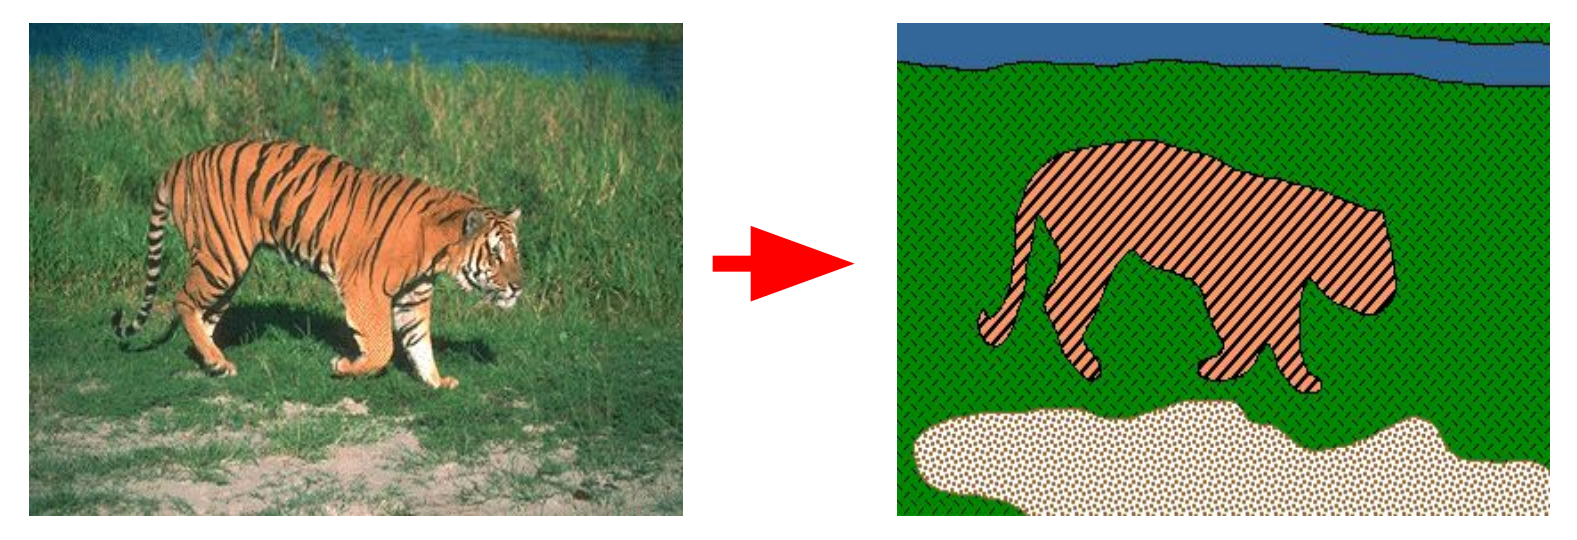
\includegraphics[width=0.75\linewidth]{cv/segmentation-tiger.png}
        \caption{Illustration of high-level image segmentation}
        \label{fig:segmentation-tiger}
    \end{figure}

    By combining individual pixels into groups, image segmentation allows for faster, more efficient image processing. It also allows for more advanced image processing with less computation. Image segmentation is widely utilized in various applications, such as medical imaging, where it assists in identifying tumors or anatomical structures, and in autonomous vehicles, where it helps recognize pedestrians, road signs, and other vehicles. By accurately separating objects from the background, image segmentation enhances the performance of machine learning algorithms and improves decision-making processes. 

    \subsection{Techniques of Segmentation}
    An important concept in image segmentation is \textbf{superpixels}. The term superpixels refers to smaller collections of pixels that are grouped together for a shared characteristic, such as color or texture. The model then is able to treat each superpixel as its own pixel, drastically reducing the amount of data taken in by the model. This reduction in the number of segments that need to be processed leads to more efficient algorithms. \newline

    Superpixels are grouped in several ways. Superpixels are designed to maintain the spatial distance and positioning of their pixels. Therefore spatial coherence is a key factor in the creation of superpixels, meaning that adjacent pixels are more likely to be included in the same superpixel. Additionally, superpixels can be formed through same-color grouping, where pixels with similar color values are clustered together, allowing for the identification of regions that share visual characteristics. Another approach is the grouping of pixels with the same texture, which focuses on the texture features of pixels, clustering them based on patterns and variations in surface properties. These different grouping methods enhance the ability of superpixels to capture meaningful segments of an image, facilitating more efficient and accurate image analysis. \newline

    Segmentation is also used to identify separate entities in images, entities that are larger than a few pixels. There are two main entity classes in segmentation, \textbf{things} and \textbf{stuffs}. Things are objects in images - people, structures, animals, etc. Things have characteristic shapes and have relatively little variance in size. Stuff, on the other hand, refers to classes with amorphic shapes, entities that are fluid and have no characteristic shapes. Sky, water, grass, and other backgrounds are typical examples of stuff. Stuff also doesn't have countable, individual instances, like things two. A blade of grass and a field of grass are both grass, but a bear and fives bears are not both a bear. There are some entities that, under certain image conditions, can be both things or stuff. For example, a large group of people can be interpreted as multiple ``persons” — each a distinctly shaped, countable thing — or a singular, amorphously shaped ``crowd”. \break

    The simplest method of entity segmentation is \textbf{semantic segmentation}. This method assigns a semantic class to each pixel, but does not identify classes or differentiate between thing and stuff classes. Semantic segmentation focuses on drawing boundaries between objects but does not assign labels to them or identify different instances of the same object. Other more complex methods of segmentation are \textbf{instance segmentation} and \textbf{panoptic segmentation}. To learn more about segmentation, see \href{https://tinyurl.com/7kz8dkhu}{IBM Image Segmentation}.
\end{flushleft}

\vspace{10px}
\begin{questionbox}
    \textbf{Synthesis Questions:}
    \begin{enumerate}    
        \item How do superpixels enhance the efficiency of image segmentation algorithms?
        \item In what scenarios might an entity be classified as both a ``thing" and ``stuff" in image segmentation? How might this dual classification impact the effectiveness of semantic segmentation methods?
    \end{enumerate}
    \vspace{1px}
\end{questionbox}

\section{When to Use Computer Vision}
\begin{flushleft}
    \large Computer vision is a field with a long history and many decades of research put into it. People have been working on these problems long before the recent waves of deep learning and machine learning. As such, it is worth digging deep into CV literature to find the best and most efficient model or architecture for your specific task. Some tools created with computer vision in mind (i.e. CNNs) can also be used in non-CV tasks if you want to leverage spatial information within your data.
\end{flushleft}

\section{Conclusion (CV)}
\begin{flushleft}
    \large 
    This section covered some of the fundamental concepts within computer vision. By leveraging techniques like Convolutional Neural Networks (CNNs) and self-supervised learning, we’ve learned how machines can mimic human vision, identifying objects, segmenting images, and even understanding complex scenes. This is no small feat; it means computers can learn to see and interpret visual information, making them more intuitive and responsive to our needs. This deep dive reveals just how crucial CV is for making sense of the visual world around us in the modern era. Computer vision serves as a bridge between the raw data captured by cameras and the meaningful insights we derive from those images. It plays a vital role in our increasingly digital lives, impacting everything from social media filters to advanced security systems.  \break
    
    Understanding these methods is key because they enable computers to perform tasks that once seemed out of reach, like accurately detecting tumors in medical imaging or helping autonomous vehicles navigate safely. For instance, in healthcare, CNNs can analyze scans and X-rays, significantly reducing the time it takes to identify critical conditions, ultimately leading to faster diagnoses and better patient outcomes. Similarly, in the realm of autonomous driving, computer vision allows vehicles to recognize pedestrians, road signs, and obstacles in real-time, enhancing safety and efficiency on the roads. These advancements not only improve operational capabilities but also build trust in technology that plays such a significant role in our lives.
\end{flushleft}
